% =============================================================================
% COPYRIGHT AND DISCLAIMER
% =============================================================================
% This file is provided as a convenience template for competition participants.
% By using it, you accept full responsibility for compliance with all applicable
% copyright, licensing, and usage rules of the Association for Computing
% Machinery (ACM) and of any LaTeX packages you load (including, without
% limitation, the "acmart" document class and related ACM materials).
%
% Consult ACM's official publication, template, and copyright policies before
% using this setup for any purpose other than this competition. Do not assume
% that this template may be reused, redistributed, or submitted elsewhere
% without independently verifying ACM's current rules.
%
% Use of the "acmart" class, the "sigconf" option, or ACM-style formatting in
% this template does NOT mean that this report, this competition, its organizers,
% or any resulting PDF is sponsored, endorsed, affiliated with, or published by
% ACM. ACM trademarks and branding remain the property of ACM.
%
% Template packages live in preamble.tex.
% Citations live in main.bib. Edit this file with your paper content.
% =============================================================================
% DRAFT (Nov 15, 2026). Numbers are for the final model, run 5981095 (soft labels, 768 px crops) with
% direction-aware grouping. Remaining open items are marked \todo{...}.
% To use in Overleaf: copy the organisers' project, replace its main.tex with this file, append
% references_to_add.bib to main.bib, and upload the three PNGs from deliverables/figures/ into a figures/ folder.

\documentclass[sigconf]{acmart}
\input{preamble}
\usepackage{tikz}
\usetikzlibrary{arrows.meta,positioning}
\newcommand{\todo}[1]{\textcolor{red}{[TODO: #1]}}   % remove all \todo{} before submitting

% Guide styling: \guideStyletrue = show gray italic hints; \guideStylefalse = omit them
\guideStylefalse      % keep on until the author block below is filled in, then switch to \guideStylefalse
% \guideStylefalse

\begin{document}

\title{Full-Resolution U-Net with Limb Normalization, Topology-Aware Loss and Direction-Aware Grouping}  % Replace this with your title
\subtitle{A Solution to the Solar Filament Segmentation Challenge 2026} % DO NOT CHANGE


\author{Sharan Rajendran}
\affiliation{%
  \city{New York City}
  \country{USA}
}
\email{sharanr1993@gmail.com}   % <- Replace with your own email

\begin{abstract}
    This report describes a solution to the Solar Filament Segmentation Challenge~2026, a Kaggle competition on automatic segmentation of solar filaments in GONG H-$\alpha$ observations. We use a U-Net with an ImageNet-pretrained ResNet-34 encoder, trained on 768\,px crops at the original 2048\,px resolution after dividing out limb darkening and the local background, with soft labels that encode how many annotators marked each pixel. The loss adds clDice and the Lovász hinge to binary cross-entropy and Dice, and a direction-aware post-processing step joins pieces of the same filament only when their ends face each other. On a held-out validation set of 141 images (217 annotator copies), the model reaches a Panoptic Quality (PQ) of 0.440 (95\% CI 0.414--0.462), above the agreement between human annotators on the same images (0.345). All code, weights and a notebook reproducing the submission are public.
\end{abstract}

\maketitle


% ==================================== %
%              INTRODUCTION            %
% ==================================== %
\section{Introduction}
    This report goes over the details of our submitted solution to the Solar Filament Segmentation Challenge~2026 \cite{filament-segmentation-2026}. The challenge, launched on July~10,~2026, is organized by the Earth-Space AI Research (ESAIR) Lab\footnote{\href{https://www.esairlab.com/home}{www.esairlab.com/}}. This challenge utilizes the MAGFiLO dataset for evaluation of the segmentation algorithms \cite{ahmadzadeh2024dataset}. Every development step was measured with the competition's metric on a local validation set, and the final pipeline is the result of that ablation (Table~\ref{tab:ablation}). Code, weights and the pipeline notebook: \url{https://github.com/sharu1993/Solar-Filament-Segmentation-Challenge-2026}.


% ==================================== %
%              METHODOLOGY             %
% ==================================== %
\section{Methodology}\label{sec:methodology}

\begin{figure*}[t]
\centering
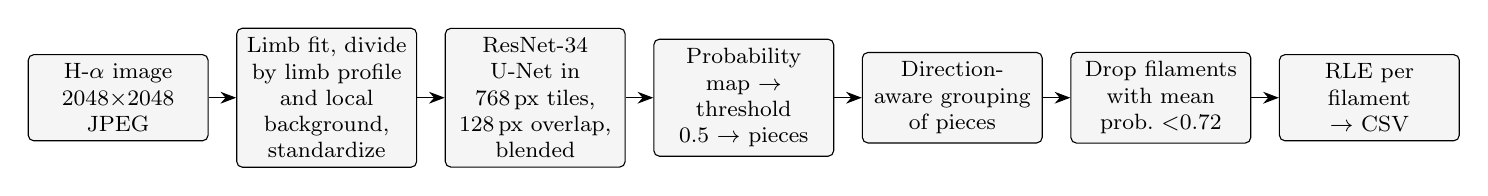
\begin{tikzpicture}[node distance=0.35cm, every node/.style={font=\footnotesize, align=center},
    box/.style={draw, rounded corners=2pt, minimum height=1.05cm, text width=2.05cm, fill=gray!8},
    arr/.style={-{Stealth[length=2mm]}}]
\node[box] (img) {H-$\alpha$ image\\2048$\times$2048 JPEG};
\node[box, right=of img] (pre) {Limb fit, divide by limb profile and local background, standardize};
\node[box, right=of pre] (net) {ResNet-34 U-Net in 768\,px tiles, 128\,px overlap, blended};
\node[box, right=of net] (thr) {Probability map $\rightarrow$ threshold 0.5 $\rightarrow$ pieces};
\node[box, right=of thr] (grp) {Direction-aware grouping of pieces};
\node[box, right=of grp] (flt) {Drop filaments with mean prob.\ $<$0.72};
\node[box, right=of flt] (out) {RLE per filament $\rightarrow$ CSV};
\foreach \a/\b in {img/pre,pre/net,net/thr,thr/grp,grp/flt,flt/out} \draw[arr] (\a) -- (\b);
\end{tikzpicture}
\caption{End-to-end inference pipeline (\texttt{deliverables/predict.py}, \texttt{pipeline.ipynb}).}
\label{fig:pipeline}
\end{figure*}

\subsection{Data and validation split}
    The training set has 707 images with 1{,}154 annotation sets; 296 images were annotated independently by 2--3 people. We hold out 20\% of the image \emph{files} (141 files, 217 annotator copies; seed 42), grouped by file so that copies of one image never fall on both sides, and score each prediction against every annotator copy, as the competition does. Only the segmentation polygons are used for training; spines, bounding boxes and class labels are never read.

\subsection{Preprocessing}
    GONG images are darker towards the limb and vary in brightness between observatories. We fit the solar disk (threshold at half the median brightness of the disk center, least-squares circle on the edge; $\sim$1--2\,px error), divide each pixel by the median brightness of its ring in a 200-ring radial profile, and then by a local background (median filter of 125\,px on a 512\,px copy, with the sky filled in by normalized Gaussian convolution so the background is not pulled down near the limb). The result is standardized per image with the median and a robust standard deviation (1.4826\,$\times$\,MAD), clipped to $\pm$5, and set to $-$5 off the disk. No position information (e.g.\ distance from disk center) is given to the network.

\subsection{Model}
    We use a U-Net \cite{ronneberger2015unet} whose encoder is an ImageNet-pretrained ResNet-34 \cite{he2016resnet}; the three color filters of the first convolution are summed into one grayscale filter. The decoder has five stages (bilinear up-sampling, concatenation with the encoder feature of the same scale, two 3$\times$3 convolutions with batch norm and ReLU), down to full resolution; a small full-resolution branch (two 3$\times$3 convolutions, 16 channels, on the input) feeds the last stage so thin structures need not be rebuilt from half-resolution features. A 1$\times$1 convolution and a sigmoid give the filament probability (24.5\,M parameters).

\subsection{Training}
    Training uses random 768$\times$768 crops of the full-resolution images, 80\% of them centered near a random pixel of a randomly chosen annotated filament so small filaments are sampled as often as large ones, with random flips, 90$^\circ$ rotations and brightness/contrast jitter. The target is a \emph{soft label}: the fraction of the image's annotators who marked each pixel (0, 1/3, 1/2, 2/3 or 1). On multi-annotator images 61\% of marked pixels are not marked by everyone (sample of 60 images), so one 0/1 mask per annotator would give contradictory targets. The loss is
    \[ \mathcal{L} = \mathrm{BCE} + \mathrm{Dice} + 0.5\,(1-\mathrm{clDice}) + 0.5\,\mathcal{L}_{\text{Lovász}}, \]
    where soft Dice counters the 0.3\% foreground, clDice \cite{shit2021cldice} rewards covering each filament's center line (thin parts count by length rather than area), and the Lovász hinge \cite{berman2018lovasz} is a smooth surrogate of the IoU on which PQ matching depends (it needs binary labels, so it uses the majority vote of the soft label). We train with Adam (learning rate $10^{-3}$, 2 warm-up epochs, cosine decay to $10^{-6}$) for 80 epochs, batch size 4, on an Apple M1 GPU ($\sim$8.3\,min per epoch, 11\,h); the checkpoint with the best validation IoU (0.546, epoch 71) is kept.

\subsection{Inference and post-processing}
    Each 2048\,px image is predicted in 768\,px tiles (3$\times$3) with 128\,px overlap, blended with weights that fall linearly towards the tile edges, so a filament crossing a tile border is continuous in the probability map. The map is thresholded at 0.5 and split into connected pieces. Pieces of one long filament are then joined by \emph{direction-aware grouping}: two pieces are merged when an end of each (the geodesic extremes of the piece) lies within 100\,px of the other's end, the outward directions at both ends are within 45$^\circ$ of the line joining them, and the mean probability along that line is at least 0.3; ends closer than 15\,px are always joined. Compared with a morphological closing (which joins anything within a fixed distance, in any direction), this joins long filaments across larger gaps without attaching unrelated nearby blobs. Finally, filaments whose mean probability is below 0.72 are dropped. All post-processing settings were chosen by a grid search on the validation set. Figure~\ref{fig:pipeline} summarizes the pipeline and Figure~\ref{fig:examples} shows examples.

\begin{figure}[t]
\centering
\includegraphics[width=\columnwidth]{figures/examples.png}
\caption{Validation images at the 25th, 50th and 85th percentile of per-image PQ (not best cases); blue: annotation, orange: prediction.}
\label{fig:examples}
\end{figure}


% ==================================== %
%              EVALUATION              %
% ==================================== %
\section{Evaluation}\label{sec:evaluation}

\subsection{Strategy}
    Our evaluation code computes PQ exactly as the organizers' self-evaluation notebook does: each annotator copy is an entry, a prediction matches an annotated filament when IoU\,$>$\,0.5, and $\mathrm{PQ}=\sum_{\mathrm{TP}}\mathrm{IoU}/(|\mathrm{TP}|+\tfrac12|\mathrm{FP}|+\tfrac12|\mathrm{FN}|)$. Applying the organizers' code to our validation predictions gives identical counts (941 TP, 365 FP, 652 FN). Uncertainties are 95\% bootstrap intervals over the 141 validation images (2{,}000 resamples, all annotator copies of an image kept together). As a reference, we scored each annotator against the others on the 48 validation images with two or more annotators.

\begin{table}[t]
\caption{Validation PQ by development step (each step adds to the previous one; best post-processing setting per model).}
\label{tab:ablation}
\small
\begin{tabular}{lcccc}
\toprule
Step & PQ & SQ & RQ & TP / FP / FN \\
\midrule
U-Net from scratch, 1024\,px & 0.277 & 0.633 & 0.437 & 680 / 839 / 913 \\
+ augmentation, longer training & 0.346 & 0.652 & 0.532 & 851 / 758 / 742 \\
+ ImageNet ResNet-34 encoder & 0.395 & 0.661 & 0.598 & 996 / 742 / 597 \\
+ 2048\,px, cosine schedule & 0.399 & 0.670 & 0.595 & 1035 / 851 / 558 \\
+ confidence filter ($\geq$0.92) & 0.413 & 0.672 & 0.614 & 977 / 615 / 616 \\
+ full-res branch, limb norm. & 0.405 & 0.674 & 0.602 & 981 / 686 / 612 \\
+ clDice + Lovász ($\geq$0.72) & 0.426 & 0.674 & 0.631 & 922 / 406 / 671 \\
+ direction-aware grouping & 0.433 & 0.676 & 0.640 & 951 / 428 / 642 \\
+ soft labels, 768\,px crops & \textbf{0.440} & 0.678 & 0.649 & 941 / 365 / 652 \\
\midrule
Annotator vs.\ annotator$^{*}$ & 0.345 & 0.629 & 0.548 & -- \\
\bottomrule
\end{tabular}\\[2pt]
\footnotesize{$^{*}$48 validation images with 2+ annotators (208 ordered pairs).}
\end{table}

\begin{table}[t]
\caption{Final model on the validation set, with 95\% bootstrap intervals.}
\label{tab:final}
\small
\begin{tabular}{lc}
\toprule
Metric & Value \\
\midrule
PQ & 0.440 (0.414--0.462) \\
SQ (mean IoU of matches) & 0.678 (0.671--0.684) \\
RQ (detection F1) & 0.649 (0.614--0.681) \\
Mean Dice of matched pairs & 0.805 \\
Mean Dice of whole-image masks & 0.673 \\
One-to-many / many-to-one filaments & 56 / 45 \\
Recall $<$500 / 500--1500 / 1500--5000 / $\geq$5000\,px & 0.34 / 0.60 / 0.67 / 0.68 \\
\bottomrule
\end{tabular}
\end{table}

\subsection{Results}
    Table~\ref{tab:ablation} shows the effect of each step. The pretrained encoder mainly reduced fragmentation; full resolution recovered small filaments. The full-resolution branch and limb normalization, tested together, scored slightly lower on their own, but the loss change on top of them gave the largest single gain: false positives fell from 686 to 406 for 59 fewer matches. The new loss also makes the model less over-confident (median probability inside correct predictions 0.82 instead of 0.96), which moved the useful confidence cut-off from 0.92 to 0.72. Direction-aware grouping added 29 matches for 22 false positives without retraining. Soft labels with 768\,px crops removed another 63 false positives (mostly predictions overlapping no annotated filament, 145\,$\rightarrow$\,90) for 10 fewer matches and raised the recall of large filaments (0.61\,$\rightarrow$\,0.68); both were changed in the same run. The PQ gain over the previous model is +0.007 (paired bootstrap 95\% CI $-$0.005 to +0.020), within the noise of a 141-image validation set. Ideas that did not help: test-time augmentation (+0.001), larger inference tiles, dilating predictions, hysteresis thresholding, and an ensemble of two models.

    Table~\ref{tab:final} gives the final scores. The model is above annotator--annotator agreement (Table~\ref{tab:ablation}): annotators often disagree on outlines and on whether a structure is one filament or two (Figure~\ref{fig:annotators}), and a model trained on all copies lands near their consensus.

\begin{figure}[t]
\centering
\includegraphics[width=\columnwidth]{figures/annotators_vs_model.png}
\caption{The same region annotated by three people and predicted by the model.}
\label{fig:annotators}
\end{figure}

\subsection{Strengths, weaknesses and improvements}
    \emph{Strengths:} one model, no ensemble or test-time augmentation; full-resolution predictions that keep thin filaments; no position prior; a local metric verified against the organizers' code; inference runs on a laptop. \emph{Weaknesses:} 73\% of the remaining false positives are \emph{near misses}, predictions on the right filament with IoU\,$\leq$\,0.5: 63\% of these cover only part of a long filament (more than half of them because it was predicted as several pieces), 16\% have IoU just under 0.5, 13\% merge two annotated filaments and 8\% spill past the outline. On images with several annotators, 64\% of near misses match \emph{another} annotator's filament (IoU\,$>$\,0.5), so much of this error is label disagreement. Recall is lowest for small filaments (0.34 below 500\,px) and near the limb (6 of 27). Post-processing was tuned on the validation set, and we used a single split and seed. \emph{Improvements:} a loss that up-weights each filament's center line (computed from the masks) to discourage gaps, since split filaments are the largest single cause of near misses; an instance-balanced loss so that each filament counts equally, as in PQ; and a term that separates neighboring filaments.


% ==================================== %
%            ACKNOWLEDGMENT            %
% ==================================== %
\section{Acknowledgment}\label{sec:acknowledgment}
    % Do not change
    The organization of the Filament Segmentation Challenge 2026 is partially supported by the U.S. National Science Foundation (NSF) under Grant No. 2209912 and 2433781, directorate for Computer and Information Science and Engineering (CSE), and Office of Advanced Cyberinfrastructure (OAC), and Grant No. 2511630, AST Division Of Astronomical Sciences and MPS Directorate for Mathematical and Physical Sciences.

    The Filament Segmentation Challenge 2026 is sponsored by the U.S. National Science Foundation (NSF) National Solar Observatory (NSO). 

    This work utilizes GONG data obtained by the NSO Integrated Synoptic Program, managed by the National Solar Observatory, which is operated by the Association of Universities for Research in Astronomy (AURA), Inc. under a cooperative agreement with the National Science Foundation and with contribution from the National Oceanic and Atmospheric Administration. The GONG network of instruments is hosted by the Big Bear Solar Observatory, High Altitude Observatory, Learmonth Solar Observatory, Udaipur Solar Observatory, Instituto de Astrofísica de Canarias, and Cerro Tololo Interamerican Observatory.

\bibliographystyle{ACM-Reference-Format}
\bibliography{main}

\end{document}
